%% Comment this out if you'd rather use another style:
%\documentclass[preprint]{JASA}

%\documentclass[preprint,trackchanges]{JASA}

%\documentclass[preprint,NumberedRefs]{JASA}

% \documentclass[reprint]{JASA}

\documentclass[reprint,NumberedRefs]{JASA}

% \documentclass[reprint,TurnOnLineNumbers]{JASA}

\usepackage[caption=false]{subfig}

\begin{document}

\title[]{Multi-resolution Analysis of Passive Cavitation Detector Data}

%% repeat as needed
\author{Max Au-Yeung}

% ie
%\author{Author One}
%\author{Author Two}
%\author{Author Three}

\affiliation{Mechanical Engineering, UCL, London, England}

\altaffiliation{}

%% for corresponding author
\email{zcemauy@ucl.ac.uk}

\begin{abstract}
Passive cavitation signals contain complex information in the time and frequency domains, making traditional use of the Fourier transform ineffective. This paper describes work to date using the wavelet packet transform to deconstruct signals. This has been combined with statistical analyses to identify key components in the signals in an attempt to identify and separate the stable and transient features in acoustic cavitation. The results indicate that further optimisation on the method is required.
\end{abstract}

\maketitle

%  End of title page for Preprint option --------------------------------- %

%% before appendix (optional) and bibliography:
\begin{acknowledgments}
This research was supported by ...
\end{acknowledgments}

\section{Introduction}
\label{sec:intro}

This section introduces the topic, its applications, and the aims and motivations behind the project.

\subsection{Acoustic Cavitation}

Cavitation refers to the growth of bubbles (spheres of gas) inside a liquid. Acoustic cavitation occurs when the bubbles are created using an acoustic source. Microscopic bubbles (microbubbles) in the fluid grow in areas of low pressure and shrink in areas of high pressure.

Acoustic cavitation primarily finds use in biomedical applications. This is because bubbles can affect fluids and tissue inside the body in a cheap and non-invasive manner. Examples include drug delivery and histotripsy. Acoustic cavitation also finds use outside of medicine in applications such as food processing and sonochemistry.

\subsection{Types of Acoustic Cavitation}

Cavitation occurs when the static pressure of the liquid falls below its vapour pressure, causing the formation of cavities filled with vapour \cite{Leighton1994}. The bubbles are either inertial (transient) or non-inertial (stable). In stable cavitation, the bubble continues to oscillate in size until the source is removed.

If the intensity of the acoustic waves is increased enough, the bubble will collapse. This is inertial cavitation. The resulting sharp increase in temperature, pressure, and the creation of free radicals can be damaging to the surrounding cells and tissue. The collapsed bubble can fragment into smaller bubbles which will serve as cavitation nuclei. These can grow into more bubbles for the process to repeat \cite{pitt2004ultrasonic}.

In general, ultrasound with low frequencies and high intensity will cause collapse cavitation. Other factors affect this, such as the size and content of the bubble.

\subsection{Project Motivation \& Aims}

This project aims to implement a method for processing experimental data gathered over a wide range of frequencies of ultrasound (300kHz – 6MHz). This range of frequencies encompasses the types of cavitation that commonly occur. This is important because the nature of the cavitation must be precisely manipulated in many of its applications \cite{pitt2004ultrasonic}. The behaviour will also change depending on several conditions e.g., temperature of liquid, gas content of liquid, intensity of ultrasound, etc. but the response of the cavitation to variation in ultrasonic frequency is especially important to analyse as one of the more easily controlled factors.

\section{Technical Background}
\subsection{Wavelet Packets}
\label{sec:Wavelet_Packets}
The wavelet packet transform can be understood as an extension of the discrete wavelet transform which in turn is an improvement on the the short-term Fourier transform (STFT). The STFT is commonly used in the field of analysing cavitation \cite{Teh2014}. This method splits the signal up using windows and computes the Fourier transform on each to add a notion of time to the transform. The equation is given by equation \ref{eq:stft}. Each set of coefficients will have a  fixed time and frequency resolution depending on the selected window size. For large windows, the frequency resolution is high while the time resolution is low. This is the other way around  for short windows.
\begin{align}
X(\tau,\omega)=\int_{-\infty}^{+\infty}{x(t)w(t-\tau)e^{-i\omega t}dt} \label{eq:stft}
\end{align}
Where $w(t)$ is a window function.

The discrete wavelet transform replaces the windowed exponential term with a wavelet (see equation \ref{eq:cwt}). Wavelets are transient, oscillating functions which can be stretched using the scale parameter. This gives the transform a higher frequency resolution for lower frequency components and a higher time resolution for lower frequency components, a much more natural way to break down a signal.

\begin{align}
F(\tau,s)=\frac{1}{\sqrt{s}}\int_{-\infty}^{+\infty}{x(t)\psi\left(\frac{t-\tau}{s}\right)dt} \label{eq:cwt}
\end{align}
Where s is the scale parameter.

The discrete wavelet transform is implemented as a series of low- and high-pass filters, given by h[n] and g[n] respectively (see figure \ref{fig:dwt_filter_bank}). Each set of coefficients is calculated using a convolution given by equation \ref{eq:dwt}. The low-pass filter produces approximation coefficients representing the amplitude of lower frequencies, while the high-pass filter produces detail coefficients, representing higher frequencies. Each set of detail coefficients correspond to a frequency range (subband) of 1 octave. The approximation coefficients correspond to the bottom end of the frequency range.

\begin{align}
y[n] = (x\ast g)[n]=\sum_{k=-\infty}^{\infty}x[k]g[n-k]\label{eq:dwt}
\end{align}

\begin{figure}
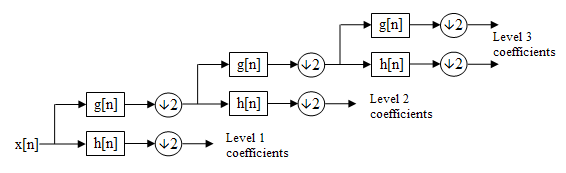
\includegraphics[width=3in]{dwt_filter_bank}
\caption{The DWT implemented as a recursive filter bank}
\label{fig:dwt_filter_bank}
\end{figure}

The discrete wavelet packet transform (DWPT) builds on this by  filtering the approximation coefficients as well as the detail coefficients at each level (see figure \ref{fig:dwpt_filter_bank}). This has the effect of improving the frequency resolution (and decreasing time resolution) at higher frequencies compared to the DWT. The more levels of transform, the narrower the frequency subbands. Learned and Willsky \cite{learned1995wavelet} note that, although the STFT can produce useful features, it does not have the same flexibility in time-frequency tiling that the packet transform does.

\begin{figure}
\begin{center}
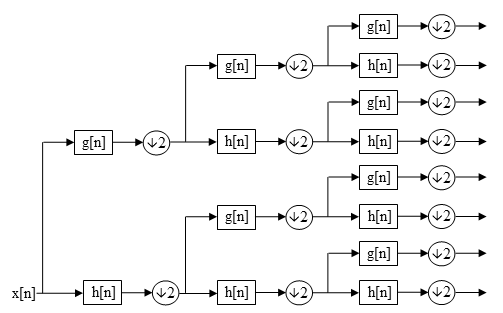
\includegraphics[width=3in]{dwpt_filter_bank}
\end{center}
\caption{The DWPT implemented as a filter bank}
\label{fig:dwpt_filter_bank}
\end{figure}

\section{Literature Review}
The methodology behind this project is based on previous works carried out in related fields. The methods used to measure cavitation, pre-process the data, select and classify features are outlined here.

\subsection{Measurement}
%compare camera measurement, ACD, PCD

\subsection{Features to Extract}
The signal from PCD is expected to contain a range of harmonics \cite{Leighton1994}. These have frequencies which are multiples of the fundamental frequency (the frequency of the ultrasound). Neppiras outlined the expected acoustic emissions for ultrasound at a range of power levels \cite{neppiras1980acoustic}. At low powers, the fundamental frequency was the only one measured. As the power was increased, but before collapse cavitation occurred, high-order harmonics were emitted by the bubbles. The emission with frequency equal to twice fundamental was prominent and had an amplitude proportional to the square of the fundamental.

Subharmonics occasionally appear. These have frequency of 1/N of the fundamental where N is an integer. This can be formed by both stable and inertial cavitation and there are many theories as to what may cause subharmonics \cite{Leighton1994}. The main theory is that they are generated by the non-linear pulsations of stable cavitation. If they are emitted by a system with only inertial cavitation, this can be explained by the prolonged expansion phase that can occur when the bubble oscillates for a few cycles before collapsing. The 1/2 and 1/3 frequency sub-harmonics are the most commonly occurring ones in acoustic cavitation.

The final component of the signal is broadband noise. There are several theories as to why this might occur. Most importantly, it is an indicator of transient cavitation. The shock wave is thought to cause this \cite{frohly2000ultrasonic}. Another possible cause for broadband noise is the bubble-to-bubble interaction, where bubbles pulsate non-periodically \cite{yasui2010numerical}. The interaction between bubbles is thought to produce harmonics and sub-harmonics as well, further increasing the difficulty in analysing clusters of bubbles. Broadband noise has the effect of increasing the intensity of each of the harmonics and sub-harmonics. The transducer will also produce some noise as well. The frequency ranges affected depends on the specifications of the transducer.

Overall, the feature extraction method must be able to separate and quantify harmonics, sub-harmonics, and broadband noise. This will make it possible to extract and classify features.

\subsection{Machine Learning}
Machine learning has been used extensively in the field of signal processing using wavelet transforms. This can be split into two major fields: supervised and unsupervised. Supervised learning relies on labelled data sets and has been used in applications such as transient detection and classification \cite{963220}, classification of EEG signals \cite{desai2020eeg}, and in fault detection \cite{rafiee2007intelligent}.

Unsupervised learning does not require labelled datasets and instead will group data points based on similarity. This is more applicable in this case where labelled data does not exist. These methods are laid out in this section.

\subsubsection{K-means}
After extracting features, the features can be classified using methods such as thresholding and clustering. K-means is a simple algorithm used for clustering. It groups the data into 'k' clusters. The aim of the algorithm is to minimise the total loss measured as the sum of the Euclidean distances between the centroid of the cluster and each point assigned to it (see equation \ref{eq:k-means}. To do this, the cluster centroids are initiated randomly and each data point is assigned to the nearest cluster. Next, the clusters are re-allocated to minimise the loss function. This process of shifting and reassigning the clusters are repeated until convergence.

\begin{align}
\Theta = \sum_{i=1}^{n}{\sum_{j=1}^{k}{\rho^{(i,j)} \lVert x^{(i)} - \mu^{(j)} \rVert^2}}
\label{eq:k-means}
\end{align}
Where Theta is the distortion (loss) function, $\rho$ is the assignment of the data point, $i$, to cluster, $j$, and $x$ and $\mu$ are the data point and cluster centroid respectively.

K-means is a non-convex optimisation problem and yields different results depending on the starting position of the clusters. There are several methods that have been developed to combat this, explained by Yiakopulos et al. \cite{yiakopoulos2011rolling}.

K-means has been combined with the wavelet transform in applications such as fault detection and EEG prediction. Both of these domains aim to categorise complex signals containing a mixture transients and harmonics. Yiakopulos et al. \cite{yiakopoulos2011rolling} applied the k-means algorithm to the problem of fault detection for rolling element bearings. Their method used two instances of K-means, one to determine whether the bearing was faulty and another to determine the nature of the fault. Each algorithm used a different set of used a different of features. They noticed that the non-convexity of k-means was a major disadvantage of the k-means algorithm and identified several techniques that have been developed to reduce the effect of this.  In their method, the centres were initialised using results from a dynamic model of the system. Shete et al. \cite{shete2013k} also used the k-means algorithm to detect the k-complex in EEG signals. This was achieved by using the k-means algorithm to compare feature of a reference k-complex signal and extracted sections of an input signal to determine whether that section contained a k-complex. This allows the training of the algorithm by providing it with examples of the feature that is sought after.

\subsubsection{Fuzzy C-means}
Fuzzy c-means is an extension of k-means where each data point is given a soft cluster assignment $0<\rho^{(i,j)}<1$ which represents the degree of membership that a given data point has to each cluster \cite{aghabozorgi2015time}. The advantage of this over k-means is that it can work better for clusters which overlap with each other, allowing for the classification of components which lie between cluster centres. The optimisation problem is the given in equation \ref{eq:c-means} where the fuzziness parameter, $m$, will cause the memberships to tend towards harder assignments as it is reduced towards 0.

\begin{align}
\Theta = \sum_{i=1}^{n}{\sum_{j=1}^{k}{\rho_{(i,j)}^m \lVert x^{(i)} - \mu^{(j)} \rVert^2}}
\label{eq:c-means}
\end{align}

Where $m$ is the fuzziness parameter.

Pan et al. \cite{pan2010bearing} used fuzzy c-means alongside the wavelet packet transform to classify bearing faults, training the algorithm on a dataset containing signals from both functional and failed bearings. The membership values allowed them to measure the extent to which a bearing had degraded, assuming that the features they extracted from the signals changed consistently between normal and degraded cases. They note that fuzzy c-means is not robust to outliers and hence developed a method to cancel out the outliers.

\subsubsection{Mixture of Gaussians}
Mixture of Gaussians is another generalisation of k-means. It aims to split a dataset into clusters represented by a user-defined number of Gaussian distributions. The advantage of this method is its ability to find non-spherical or hyper-spherical clusters in a dataset, which is shown to be applicable in this case.

\subsubsection{Self-organising Maps}
Self organising feature maps (SOFMs) are a type of neural network designed for clustering. It is able to produce clusters as a topological map of connected nodes, where neighbouring nodes share some degree of similarity. This is often used to visualise the feature space, especially with maps of lower dimensionality (often 2D or 3D).

\subsubsection{Feature Selection}
Once data is acquired using PCD, the resulting sound wave is processed using the wavelet transform (see section \ref{sec:Wavelet Packets}) to extract features. From the transform, features must be selected. Matloobi and Riahi trained a neural network to identify cavitation inside a centrifugal pump using the discrete wavelet transform to extract features. \cite{matloobi2021identification}. They used statistical features such as room mean square, kurtosis, skew, mean, and peak of the signal and the transformed data. These features are commonly used among approaches involving clustering \cite{yiakopoulos2011rolling} \cite{shete2013k}.

The DWPT is also a highly redundant transform \cite{mallat1999wavelet} meaning that many of the nodes, especially those neighbouring each other in the frequency domain, will contain similar information. There also exists a large class imbalance where very few nodes will represent the portion of the signal containing harmonic data meaning that there will be a large class imbalance in the clustering problem. Both of these issues can be solved by selecting appropriate nodes for clustering. Shannon entropy is a commonly-used approach for dealing with problem \cite{kim2012heath}. The entropy of the $i^{th}$ node of at the $j^{th}$ scale is defined in equation \ref{eq:entropy}

\begin{align}
E_i = \sum^M_{k=1}{e^i_{j,k}\log{e^i_{j,k}}}\label{eq:entropy}
\end{align}
Where the energy of each coefficient in an array containing M coefficients is:
\begin{align}
e^i_{j,k}=\frac{y^i_{j,k}}{\sum^M_{k=1}{y^i_{j,k}}}
\end{align}

\section{Methodology}
\label{sec:methodology}
This section will outline the methods used by Teh \cite{Teh2014} and Haqshenas \cite{Haqshenas_2015}.

\subsection{Classification of Features}
When the wavelet packet transform is applied on a signal, the resulting coefficients at each node correspond to the correlation of the signal with the wavelet. The coefficients at each frequency subband can be separately reconstructed into signals which combine to form the original signal. The stable and transient components of the signal tend to have greatly different frequencies, so the transform will help separate these out. Once separated, the subbands can be classified to give an indication of the presence and extent of each type of cavitation.

\subsubsection{Statistical Measures}
Haqshenas \cite{Haqshenas_2015} used statistical measures on the wavelet packet coefficients, calculating the energy, kurtosis, and crest factor at each subband. These are able to distinguish between transient and stable signals.

The energy of a subband is a measure of how much the signal is concentrated within it. Energy is calculated as the variance of the coefficients belonging to that subband (see equation \ref{eq:energy}). This is useful for separating out fundamental frequency and higher amplitude harmonics.

\begin{align}
E = \frac{1}{N}v^Tv \label{eq:energy}
\end{align}
Where $v$ is a vector containing the coefficients in a subband and N is the number of coefficients in the subband.

Kurtosis is a measure of how often outliers occur. This is calculated using the equation \ref{eq:kurtosis}. High kurtosis is used as an indicator of transient cavitation.

\begin{align}
K = \frac{E(x-\mu)^4}{\sigma^4} \label{eq:kurtosis}
\end{align}

The crest factor is the ratio between the peak value and the mean of the signal (see equation \ref{eq:crest_factor}. This measures how extreme the peaks are in the signal. A higher crest factor indicates the presence of high amplitude outliers in the signal.

\begin{align}
C = \frac{{\max{(|x|)}}^2}{x_{rms}^2} \label{eq:crest_factor}
\end{align}

These features are calculated on the wavelet coefficients.

\subsubsection{Analysis}
The statistical measures give an indication of the strength and stablity of the signal in each frequency subband, allowing for the classification of stable and transient features. This is combined with thresholding, where the features are selected based on whether their statistical measures are above or below a given value. The illustrate the effect of thresholding, a synthetic signal (see figure \ref{fig:synth_signal} was transformed (see figure \ref{fig:dwpt_synth}). This data was generated using 2 sine waves with frequencies 1 and 100Hz. A series of short, high amplitude hanning windows were added to this to represent transients. Finally, the signal was windowed. No noise has been added.

The FFT of the signal represents the transients as a range of low amplitude frequencies as shown by the low level of background noise around the two peaks. In the wavelet packet transform, the transients are more visibly separated out across different subbands and more localised time. 

Next, the subbands are reconstructed to form waves reconstructed waves with the highest energy, kurtosis, and crest factor are shown in figure \ref{fig:highest_synth}. The highest energy subband was the lowest (fundamental) frequency. The second highest energy subband (not shown here) was the one containing the other frequency of 10Hz, indicating that energy will tend to pick out the high amplitude low frequency components. The subbands with the highest kurtosis were similar to the one shown in figure \ref{fig:highest_synth}. They were frequency subbands containing only transient components, indicating that kurtosis is a good measure of transience without any noise present. Finally, the subbands with the highest crest factor picked were those remaining in the lower frequency ranges. These contained some transient components mixed with the lower frequency sine waves.

When Gaussian noise is added to the data, the highest subbands sorted by energy and crest factor tends to remain the same, but the measure of kurtosis is impacted and will tend to return similar results to the crest factor.

\begin{figure}
\begin{center}
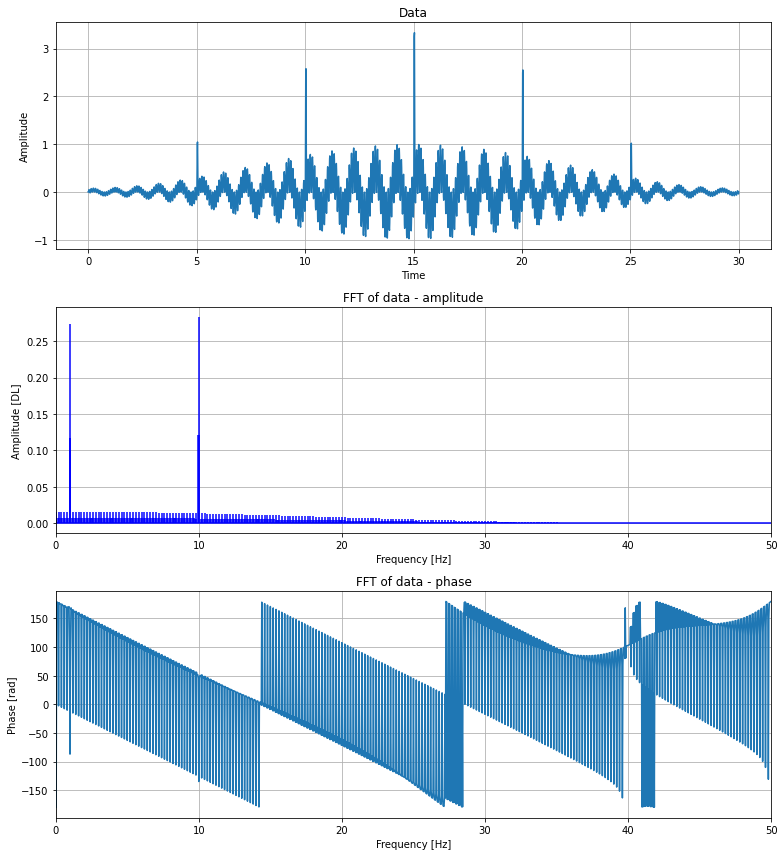
\includegraphics[width=3.5in]{synth_data}
\end{center}
\caption{synthetic data with sampling rate 100 with frequencies 1Hz and 10Hz, transient components, and noise.}
\label{fig:synth_signal}
\end{figure}

\begin{figure}
\begin{center}
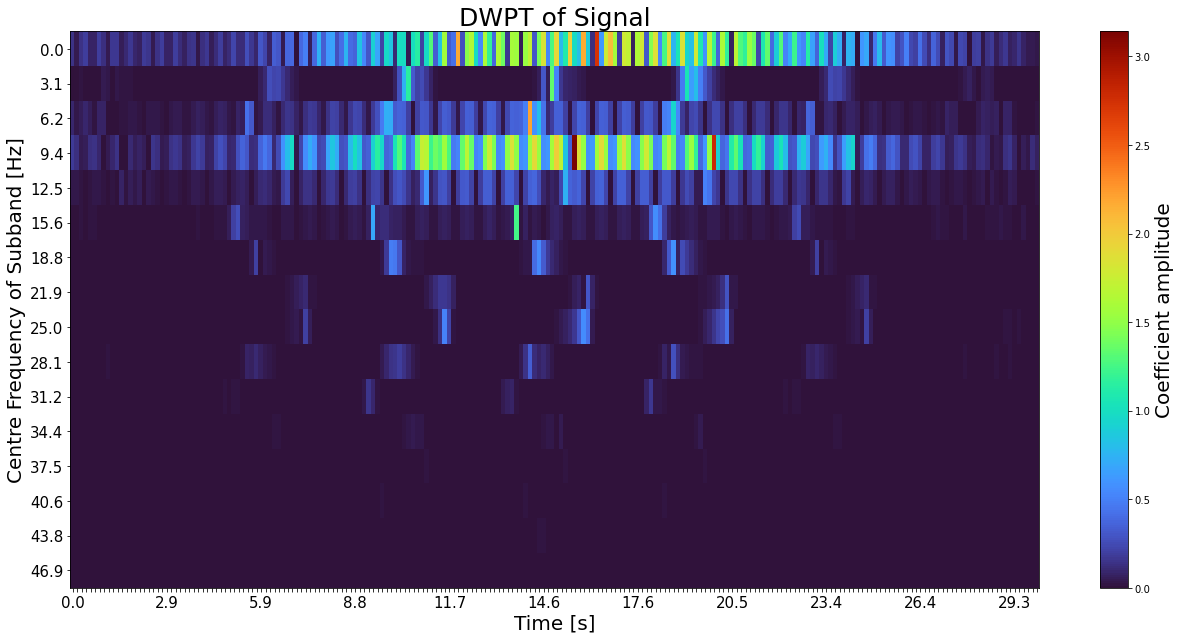
\includegraphics[width=3.5in]{dwpt_synth}
\end{center}
\caption{Heisenberg plot of a 4-level db16 DWPT of a synthetic signal in figure \ref{fig:synth_signal}.}
\label{fig:dwpt_synth}
\end{figure}

\begin{figure}
\begin{centering}
\subfloat[]{%
  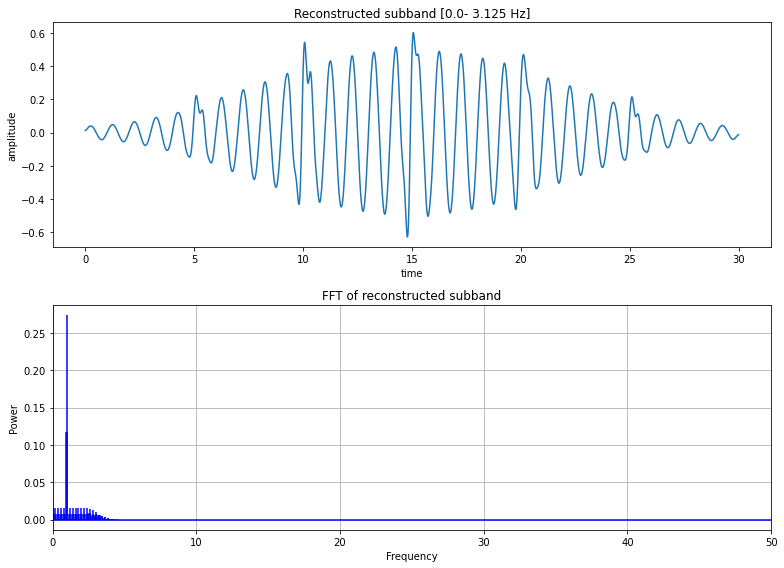
\includegraphics[clip,width=0.7\columnwidth]{highest_energy_synth}%
}
\hfill
\subfloat[]{%
  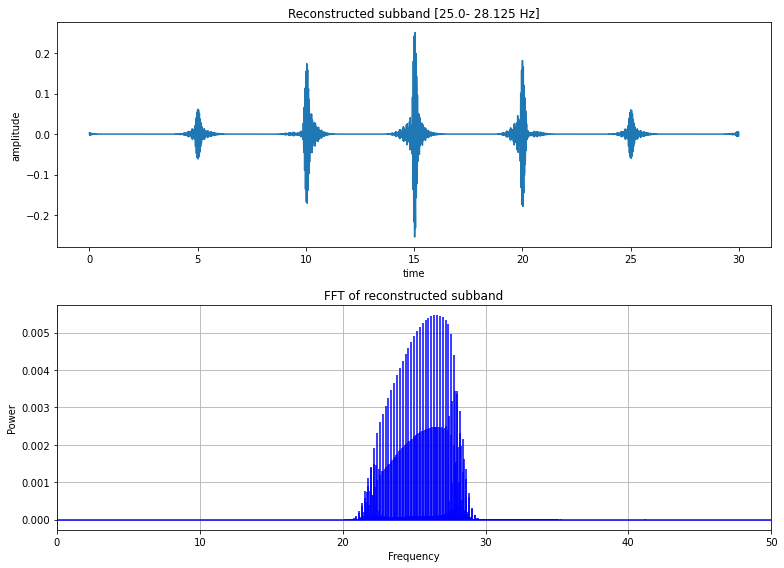
\includegraphics[clip,width=0.7\columnwidth]{highest_kurtosis_synth}%
}
\hfill
\subfloat[]{%
  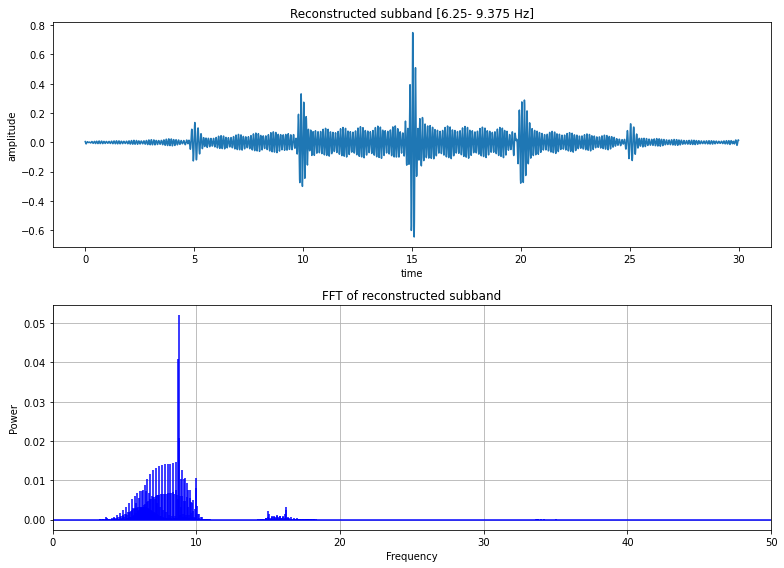
\includegraphics[clip,width=0.7\columnwidth]{highest_crest_synth}%
}
\hfill
\caption{Reconstructed subbands with highest energy (a), kurtosis (b), and crest factor (c) respectively}
\label{fig:highest_synth}
\end{centering}
\end{figure}

\section{Results}
\label{sec:results}

\section{Summary}
\label{sec:summary}
% ---------------------------------------------------------------------
% Appendix  (optional)

%\appendix
%\section{Appendix title}

%If only one appendix, please use
%\appendix*
%\section{Appendix title}

%% After first section in \appendix*,
%% \section{} the term APPENDIX will not be used.

%=======================================================
\section{References}
\bibliography{references}

%%When uploading your files to Editorial Manager,  include both the .bib and the appropriate .bst file (for author/year reference style: jasaauthoryear2.bst; for numerical style: jasanum2.bst). Both the .bib and .bst should be uploaded as the “Manuscript (TeX or Word only)” item type.


%=======================================================

\end{document}